
\documentclass[a4paper,12pt,oneside,pdflatex,italian,final,twocolumn]{article}



\usepackage[utf8]{inputenc}
\usepackage{parallel}
\usepackage{siunitx}
\usepackage{booktabs}
\usepackage{fancyhdr}

\usepackage[export]{adjustbox}
\usepackage[margin=0.5in]{geometry}
\addtolength{\topmargin}{0in}

\usepackage{libertine}
\renewcommand*\familydefault{\sfdefault}  %% Only if the base font of the document is to be sans serif
\usepackage[T1]{fontenc}







\title{BSPD 2019}
\author{arsphotographika }
\date{April 2019}

\begin{document}

\pagestyle{fancy}

\lhead{ITBA}
\rhead{3-Band-EQ-G1}


\onecolumn

\begin{figure}
  \begin{minipage}{0.47\textwidth}
    \centering
    
\includegraphics[width=.7\textwidth,left,]{logo}

  \end{minipage}
  \hfill
  \begin{minipage}{0.47\textwidth}
    \raggedleft
    \Huge \textbf{3-Band-EQ-G1}
  \end{minipage}
\end{figure}


\begin{figure}
  \begin{minipage}{0.6\textwidth}

    \section{Overview}
    \begin{itemize}
      \item Alimentación con doble fuente de contínua: $\pm 15$
      \item Entrada: $0$ a $\pm 1V$ (En condiciones normales de uso)
      \item Salida: $0$ a $\pm 15V$
      \item Frecuencias de ecualización: $98 Hz$, $1,1 KHz$ y $8,4 KHz$
    \end{itemize}


  \end{minipage}
  \hfill
  \begin{minipage}{0.4\textwidth}
    \centering
    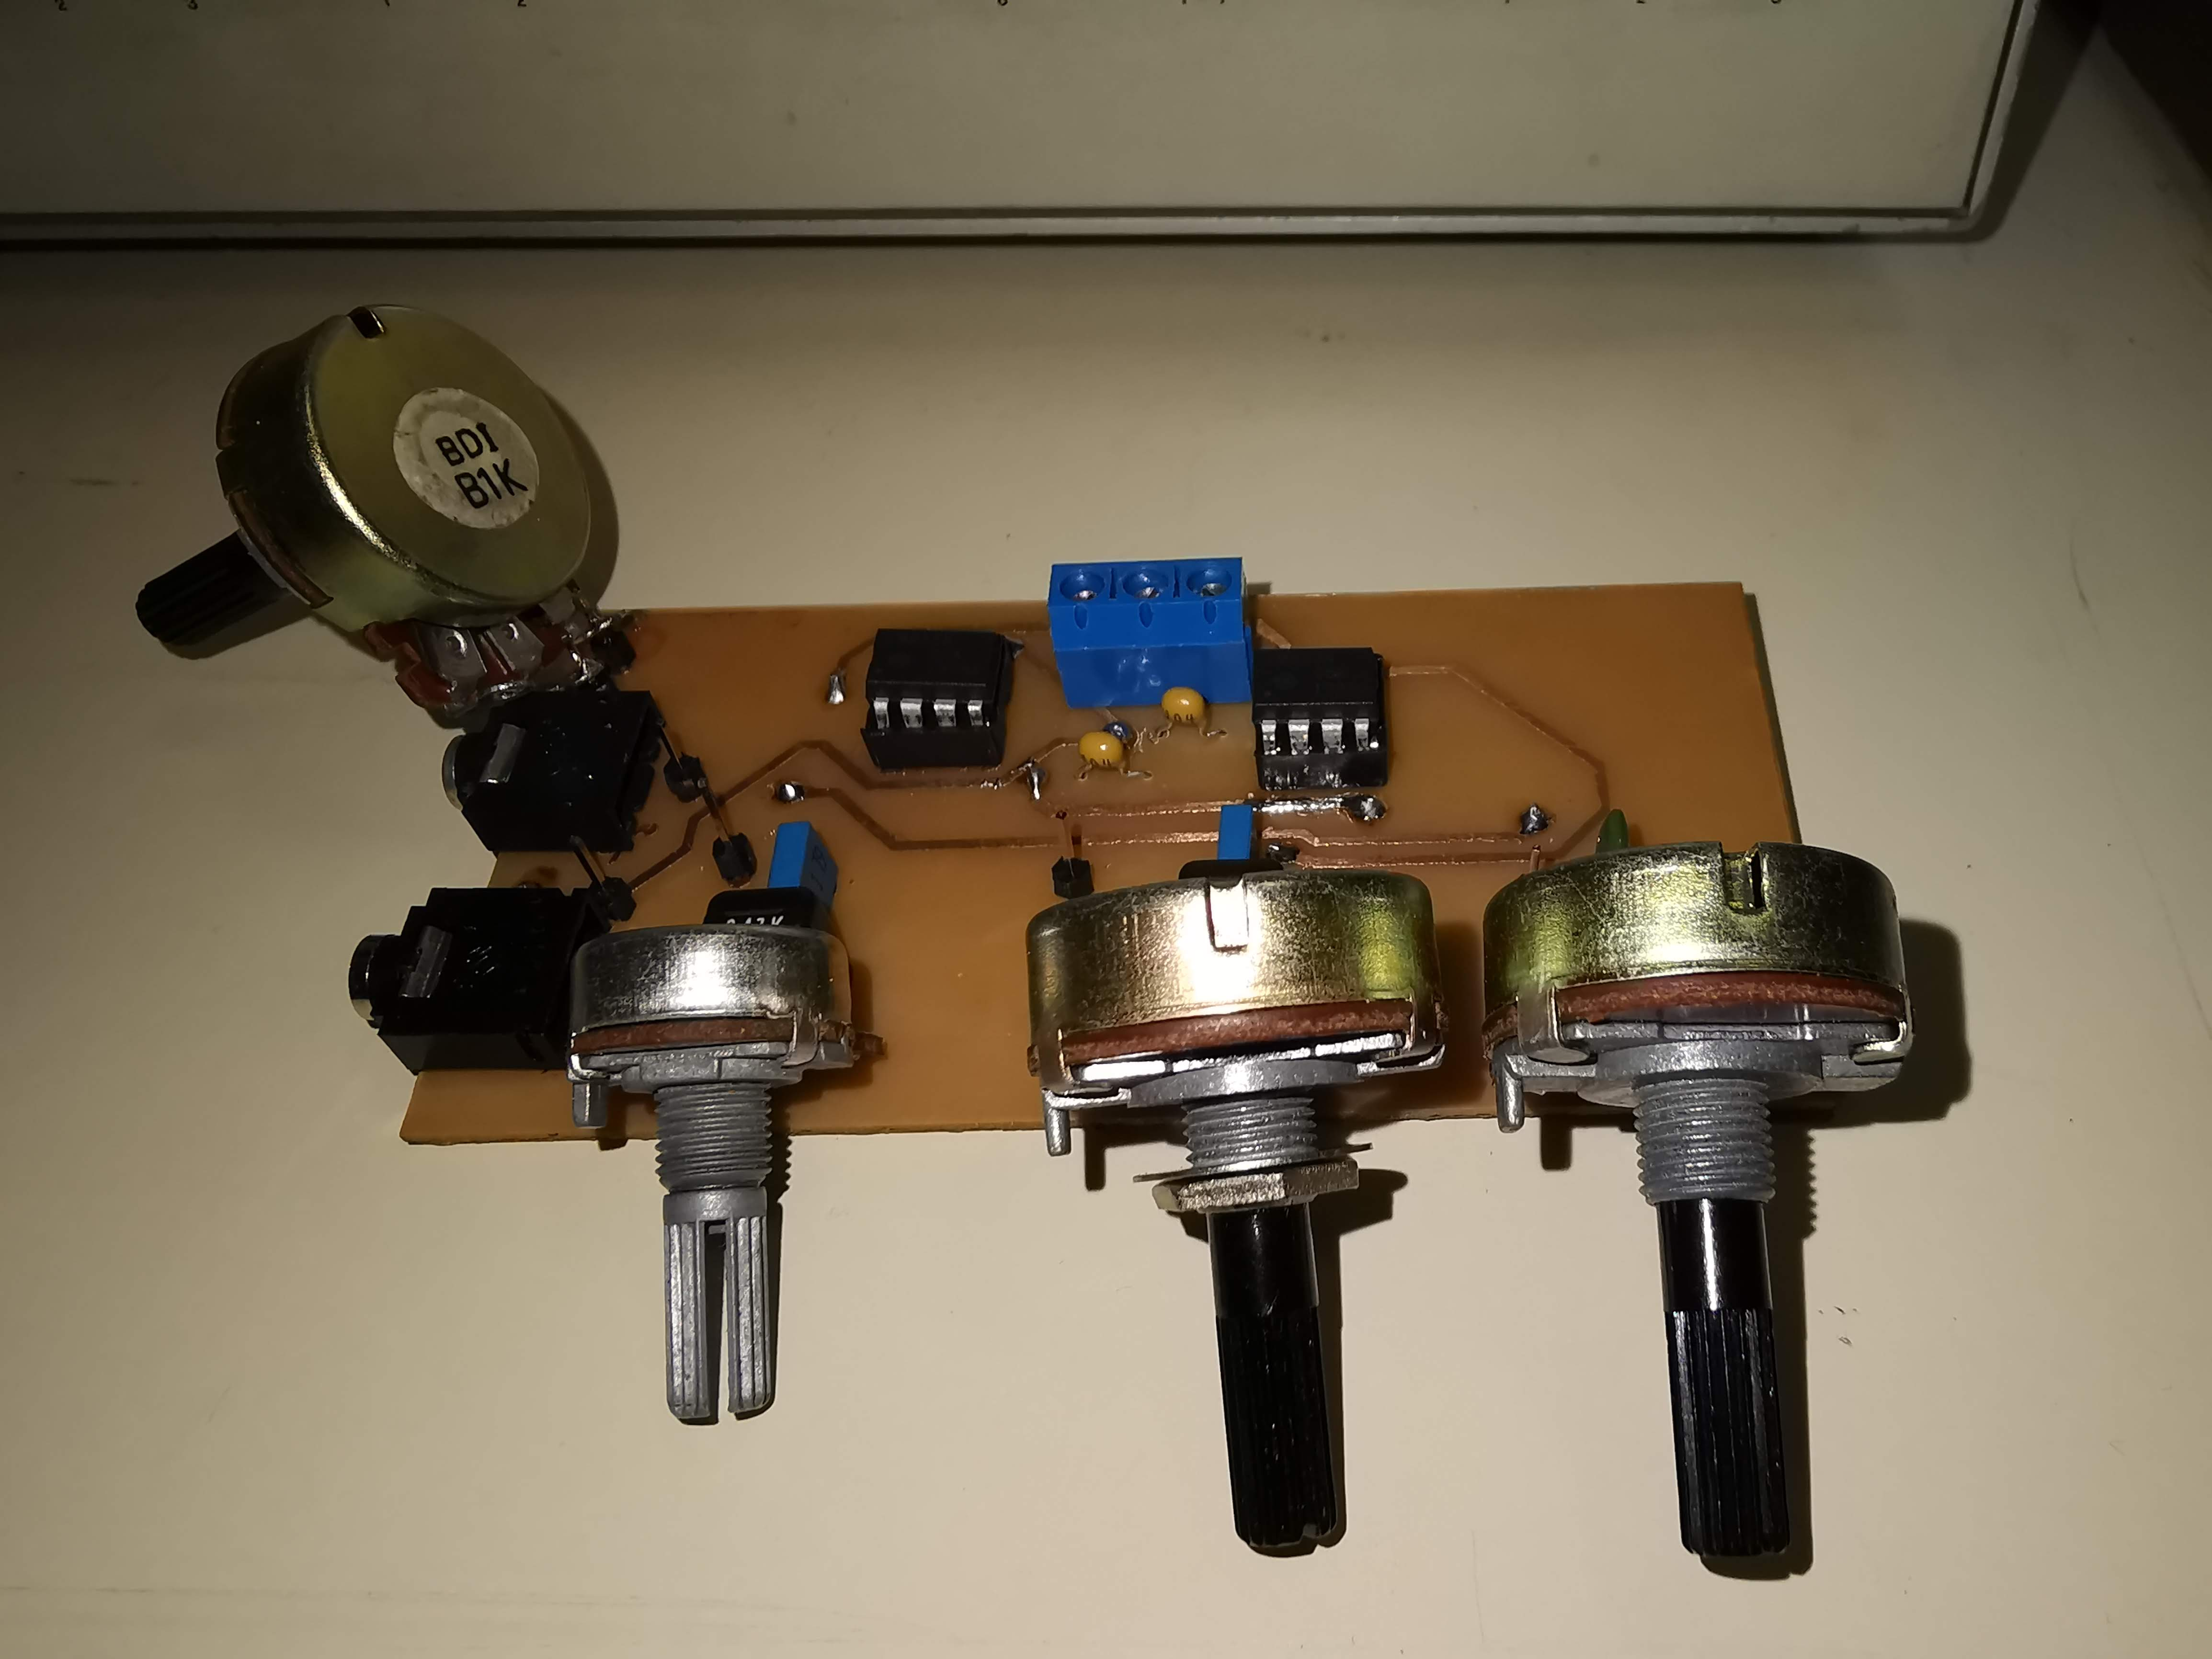
\includegraphics[width=0.9\textwidth,right]{EQ_picture}

  \end{minipage}
\end{figure}


\begin{minipage}{0.47\textwidth}
  \section{Descripción}
  Un ecualizador de tres bandas es un circuito diseñado con tres etapas de filtros con ganancia cercana a 1 para todo el espectro audible, excepto en las cercanías de la 
  frecuencia para la cual fue diseñada cada etapa.
  En otras palabras, para tres frecuencias representativas del rango audible, funciona como un pasa banda o rechaza banda, siendo su comportamiento determinado por 
  resistencias variables al alcance del usuario.\par
  Con el objetivo de lograr la mayor cobertura posible del rango audible, las frecuencias de corte de cada uno de los ecualizadores fueron diseñadas en $98 Hz$, $1,1 KHz$ y $8,4 KHz$,
  correspondientes a sonidos bajos, medios y altos, respectivamente.
  El circuito cuenta además con un control de volumen ya integrado, y, dejando de lado la alimentación, no requiere de componentes externos para su funcionamiento. \\
\end{minipage}
\hfill
\begin{minipage}{0.47\textwidth}
  \section{Cualidades}
  \begin{itemize}
    \item Amplio rango de ganancia en frecuencias bajas.
    \item Manejo independiente de las tres bandas.
    \item Bajo costo.
    \item No necesita de componentes externos.
    \item Control de volumen integrado
    \item Buena regulación de carga ($Z_{out} < 100 \Omega$)
  \end{itemize}
    
  \section{Aplicaciones}
  Controladores de audio de bajo costo donde el control de los bajos sea prioridad.

\end{minipage}

\begin{minipage}{0.47\textwidth}
  \section{Absolute maximum ratings}
  \centering
  \begin{tabular}{lcr}
    \toprule
    & Value & Unit \\
    \midrule
    $+V_{cc}$ & $+18$ & $V$ \\
    $-V_{cc}$ & $-18$ & $V$  \\
    $+V_{cc} - -V{cc}$ & $36$ & $V$ \\
    $V_{pp\_in\_max}$ & 5 & $V$ \\
    Corriente de input & $\pm 10$ & $mA$ \\
    \bottomrule
  \end{tabular}
\end{minipage}
\hfill
\begin{minipage}{0.47\textwidth}
  \section{Condiciones de operación recomendadas}
  \centering
  \begin{tabular}{lcr}
    \toprule
    & Value & Unit \\
    \midrule
    $+V_{cc}$ & $+15$ & $V$ \\
    $-V_{cc}$ & $-15$ & $V$  \\
    $V_{pp\_in\_max}$ & 1 & $V$ \\
    \bottomrule
  \end{tabular}
\end{minipage}

\raggedright

\newpage

\section{Características típicas}
\begin{minipage}{0.47\textwidth}
  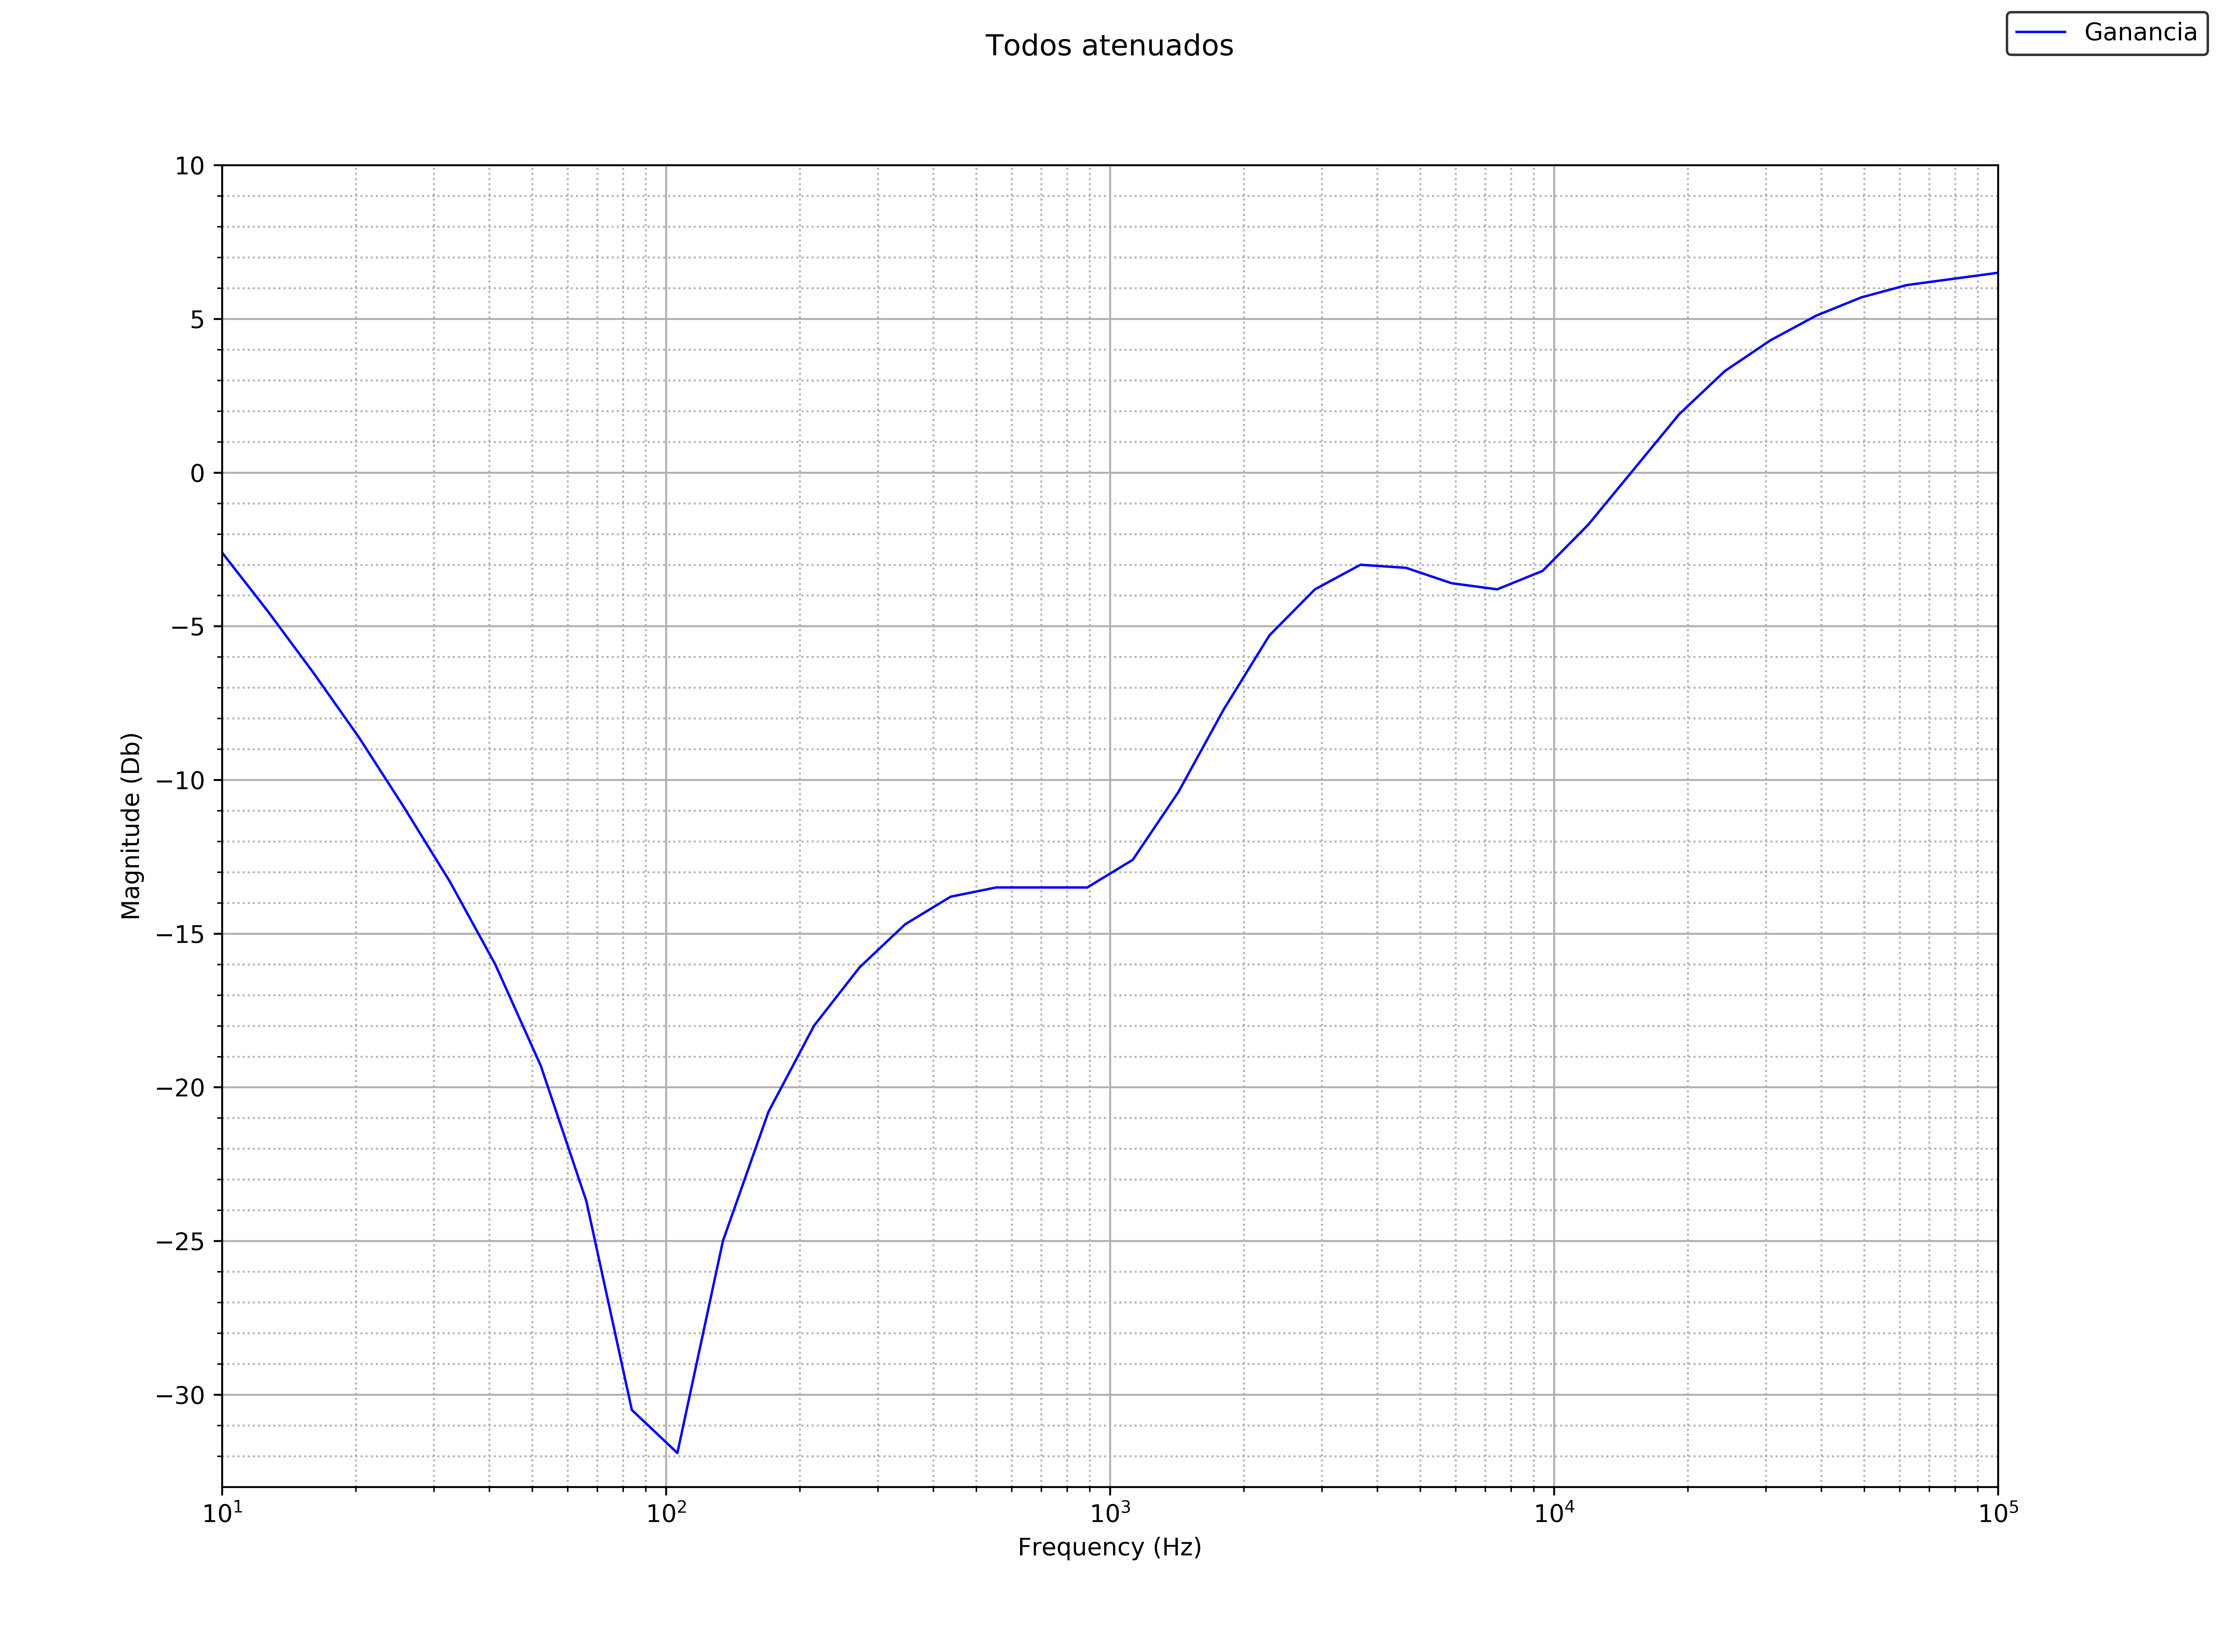
\includegraphics[width=\textwidth]{-B-M-A}
\end{minipage}
\hfill
\begin{minipage}{0.47\textwidth}
  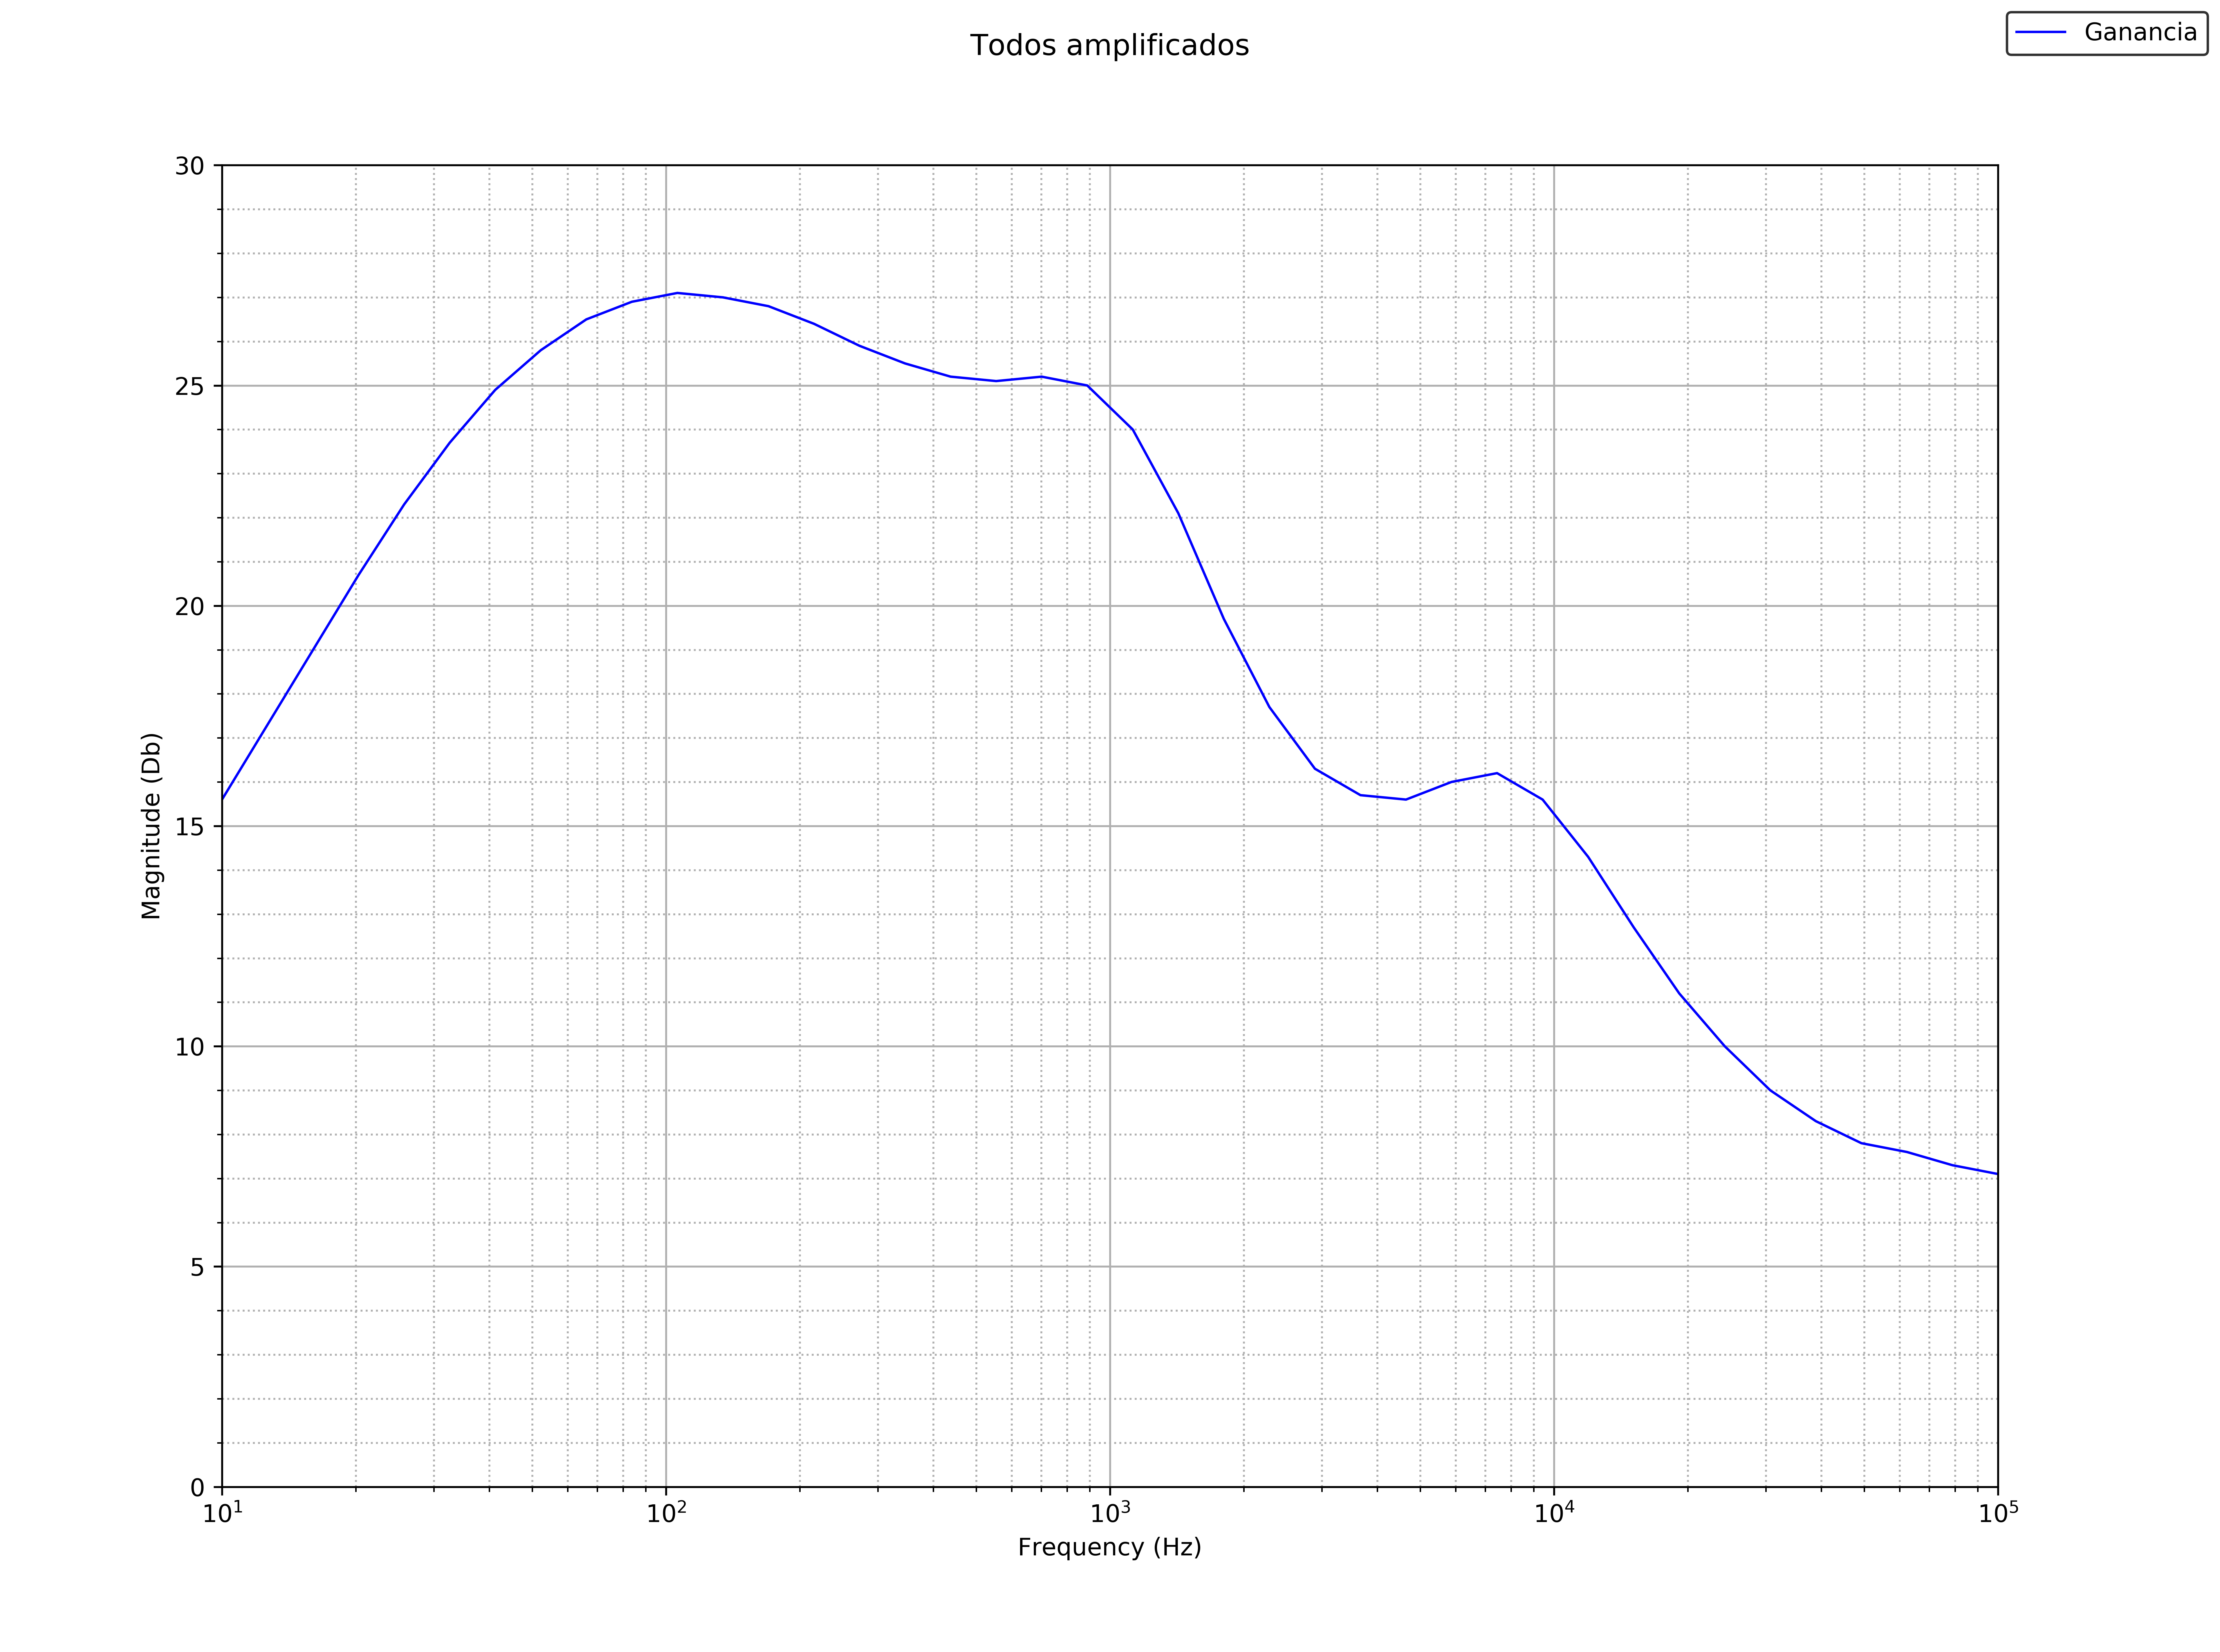
\includegraphics[width=\textwidth]{+B+M+A}
\end{minipage}

\begin{minipage}{0.47\textwidth}
  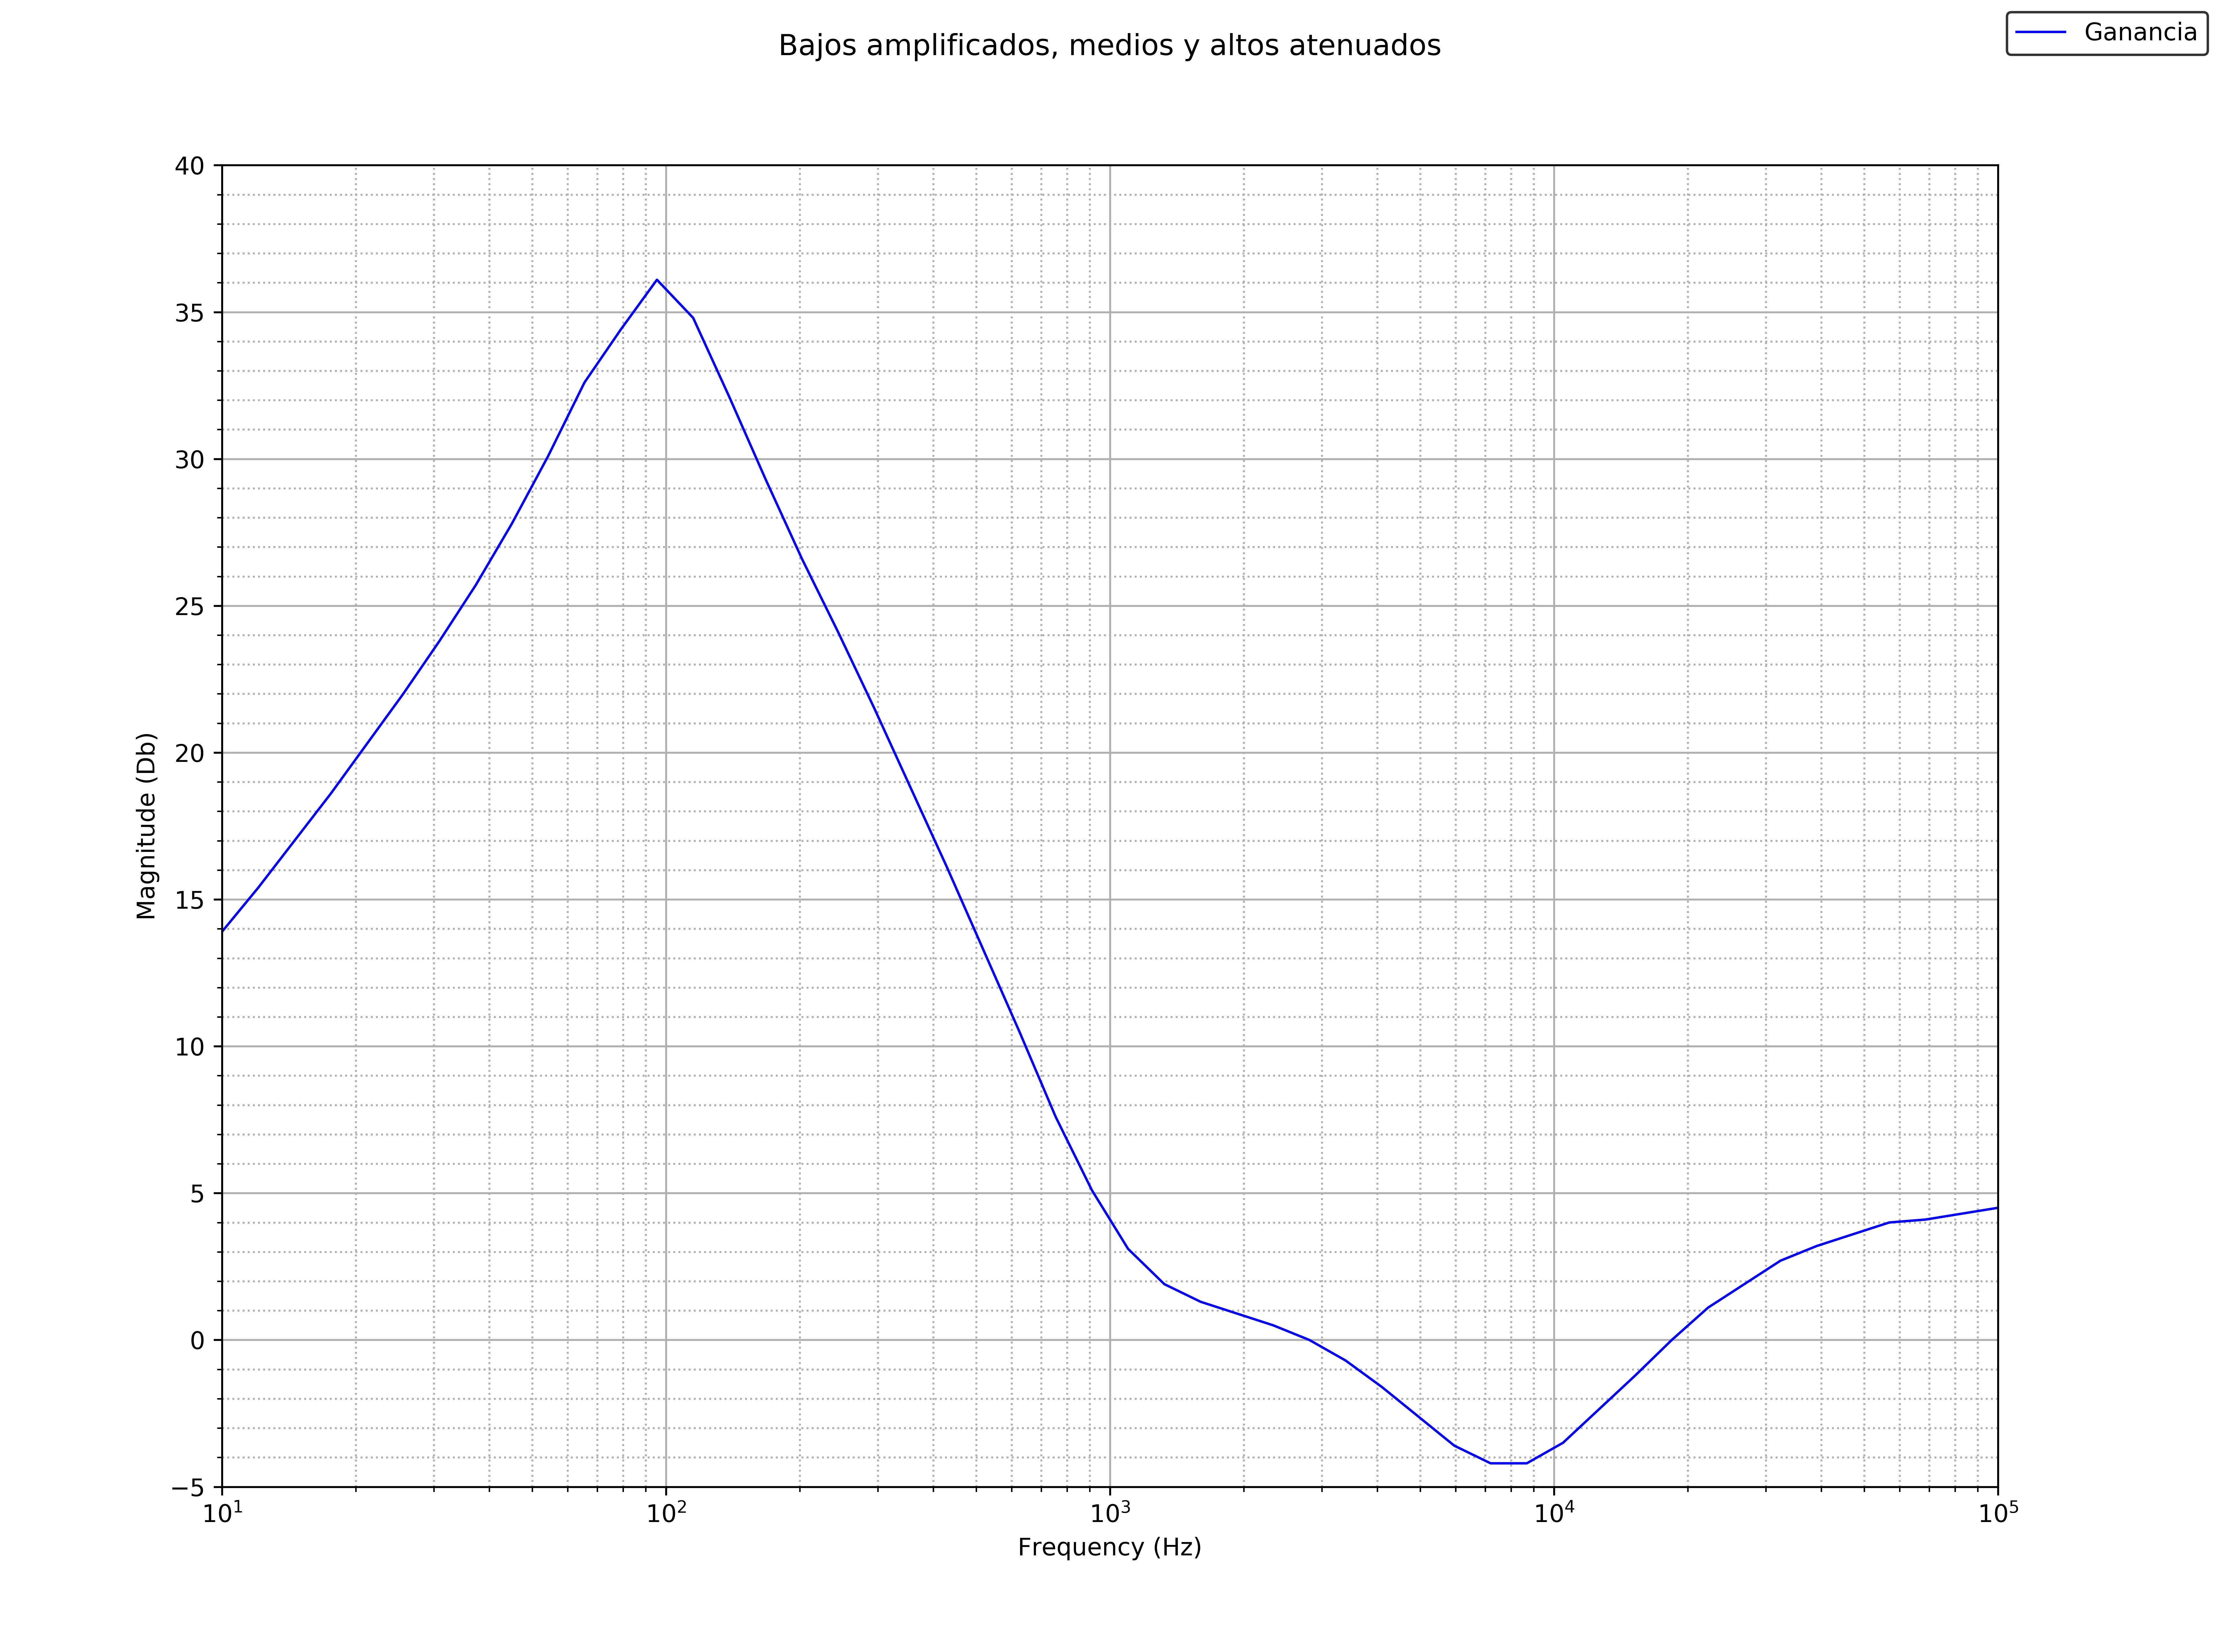
\includegraphics[width=\textwidth]{+B-M-A}
\end{minipage}
\hfill
\begin{minipage}{0.47\textwidth}
  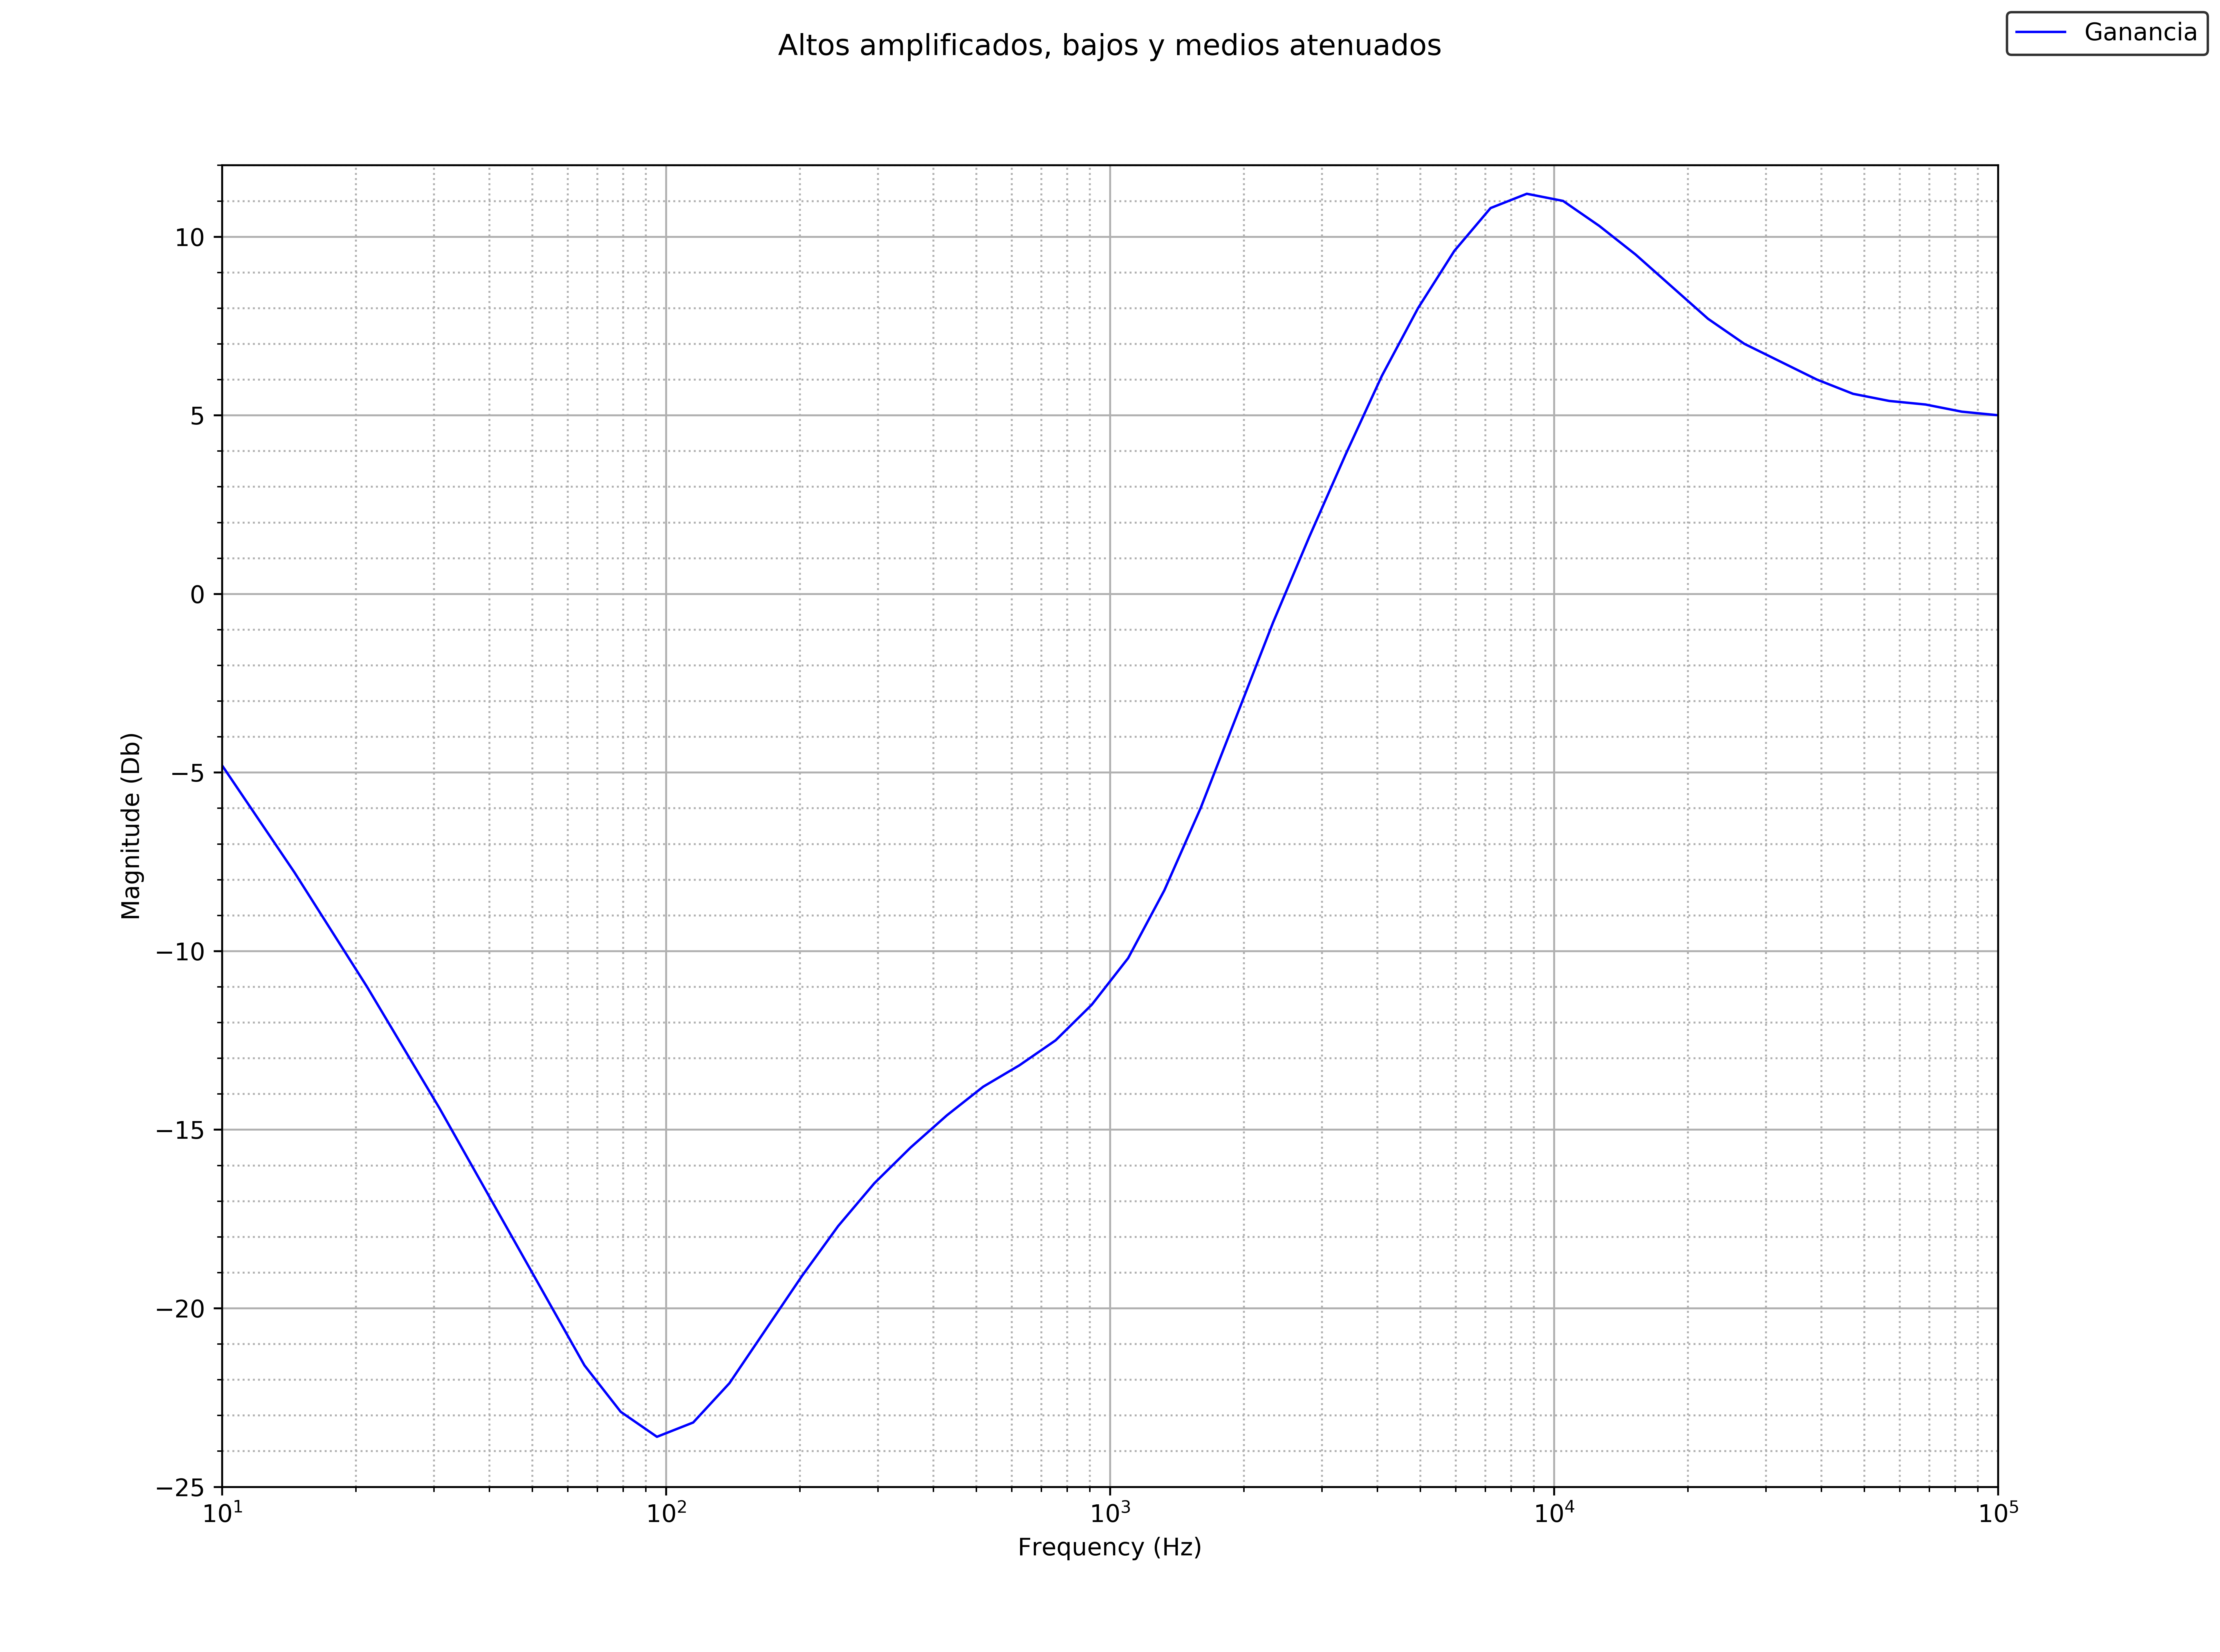
\includegraphics[width=\textwidth]{-B-M+A}
\end{minipage}

\begin{minipage}{0.47\textwidth}
  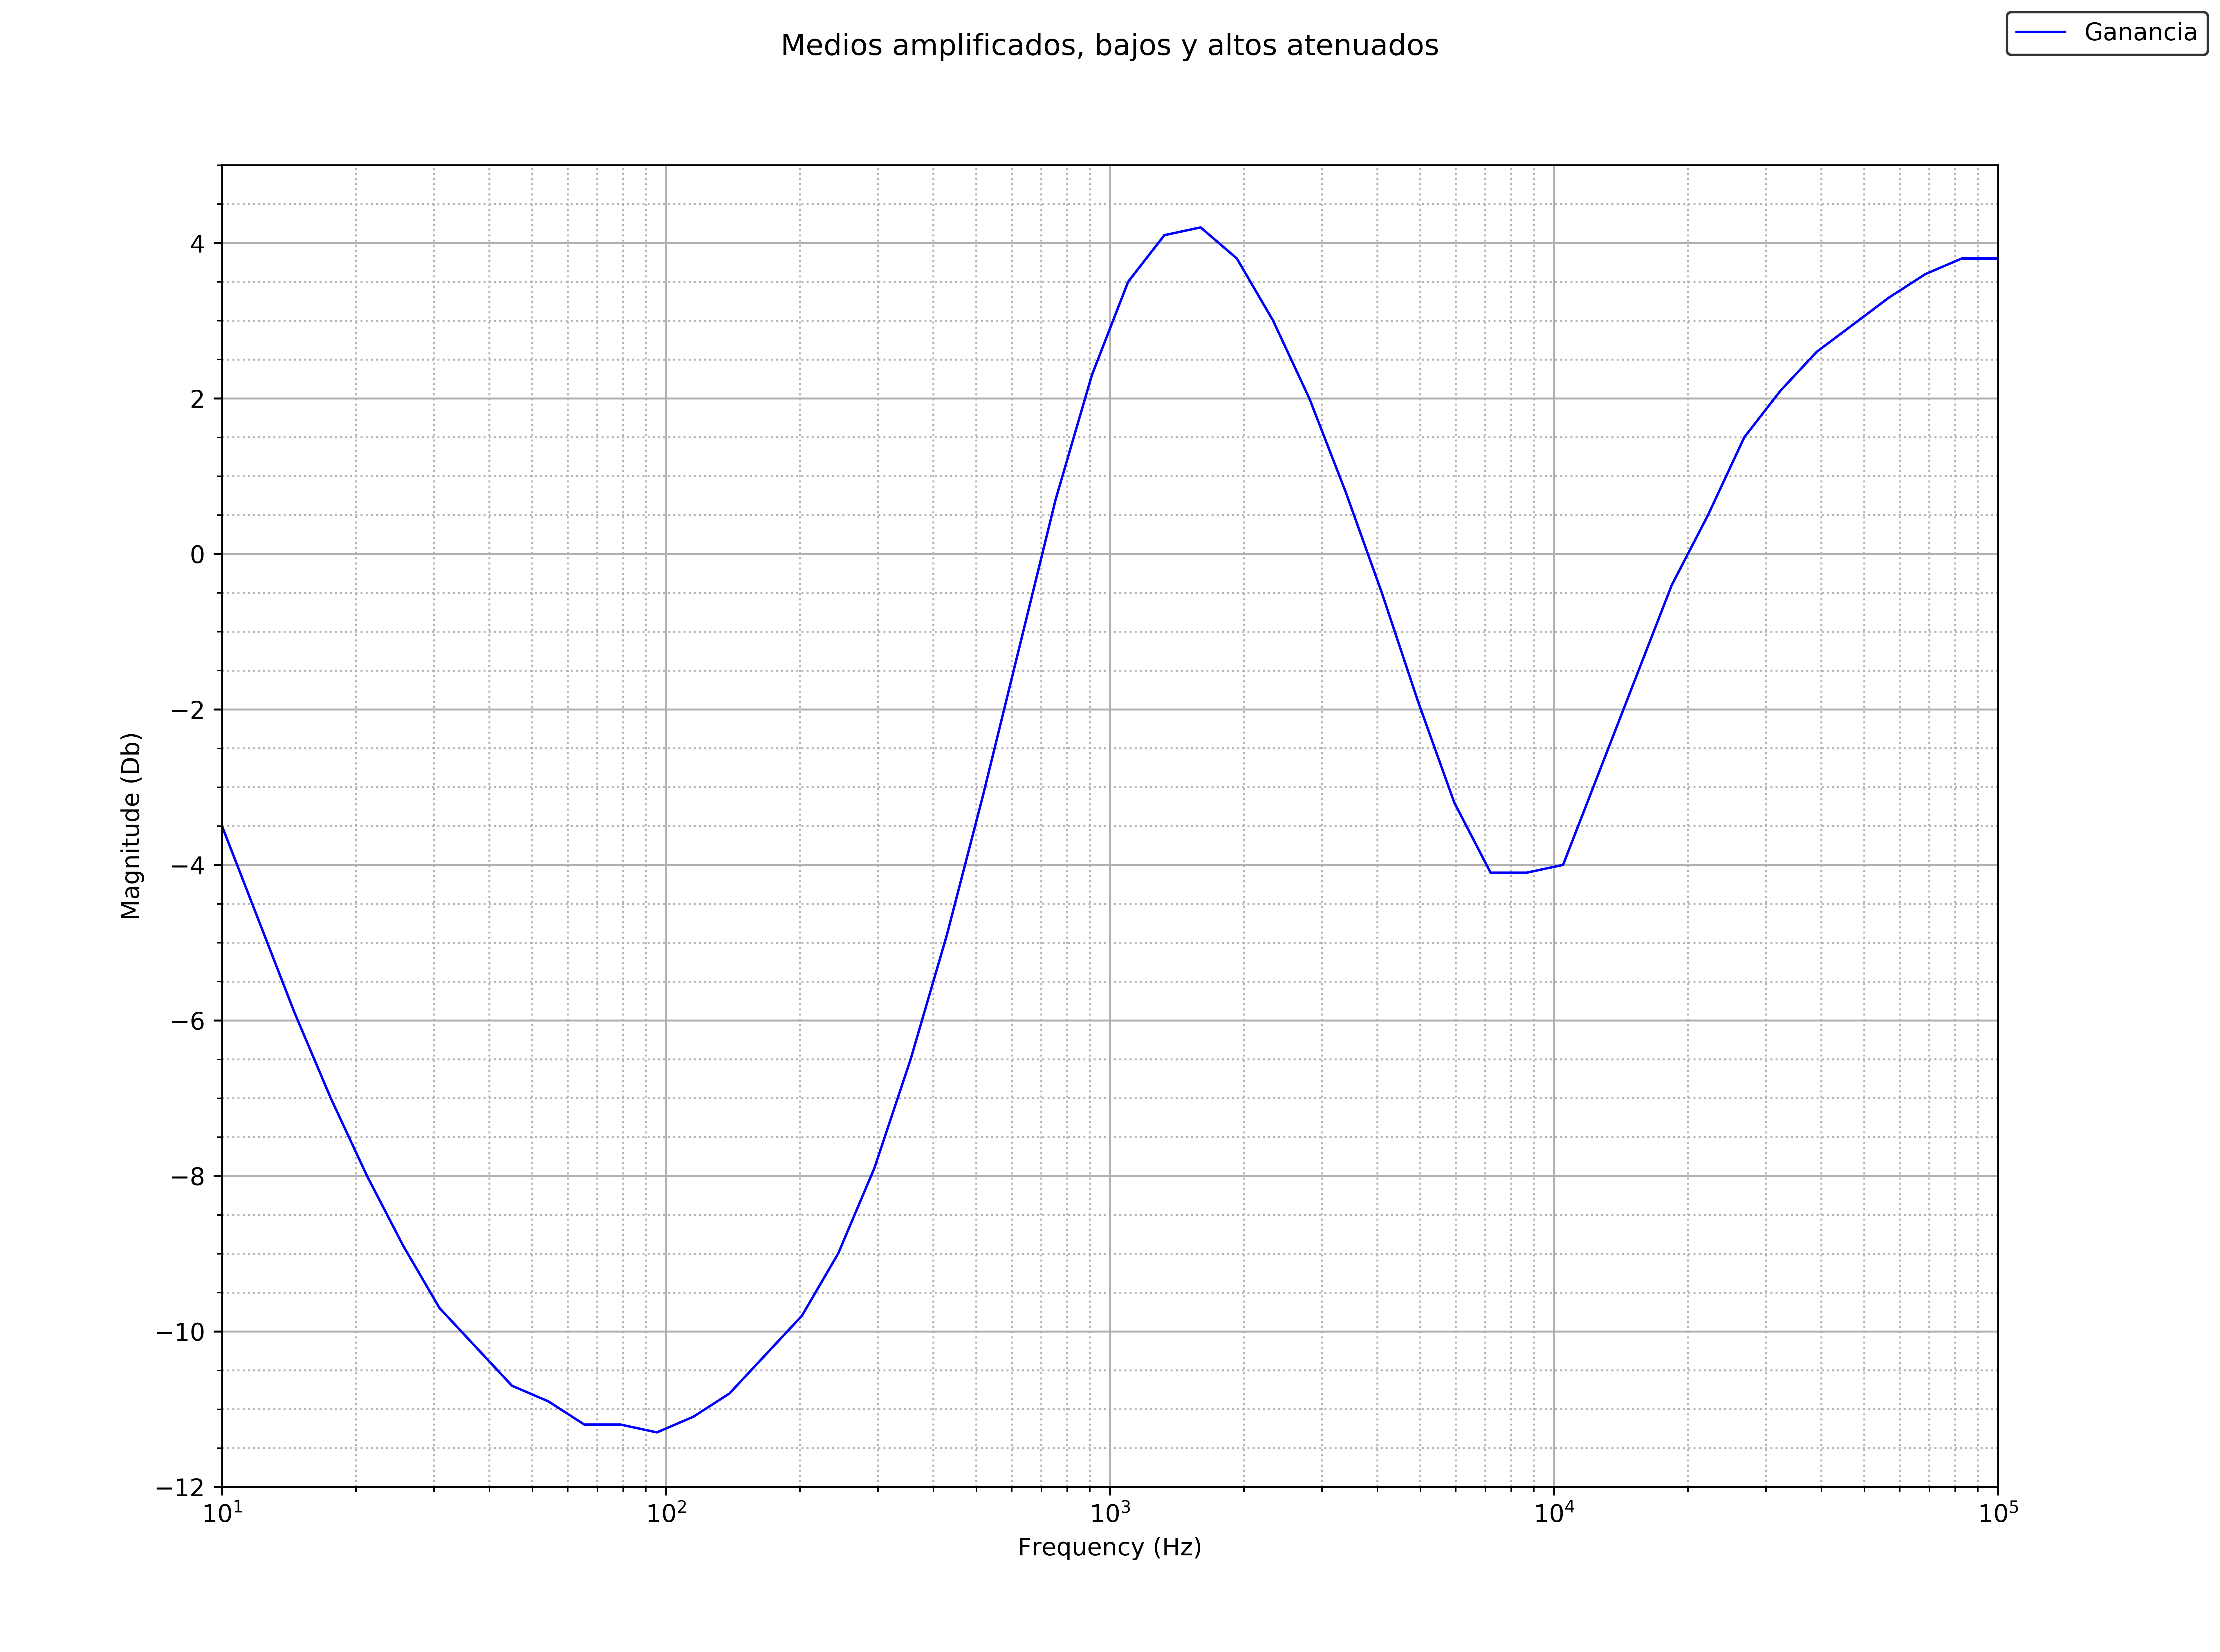
\includegraphics[width=\textwidth]{-B+M-A}
\end{minipage}
\hfill
\begin{minipage}{0.47\textwidth}
  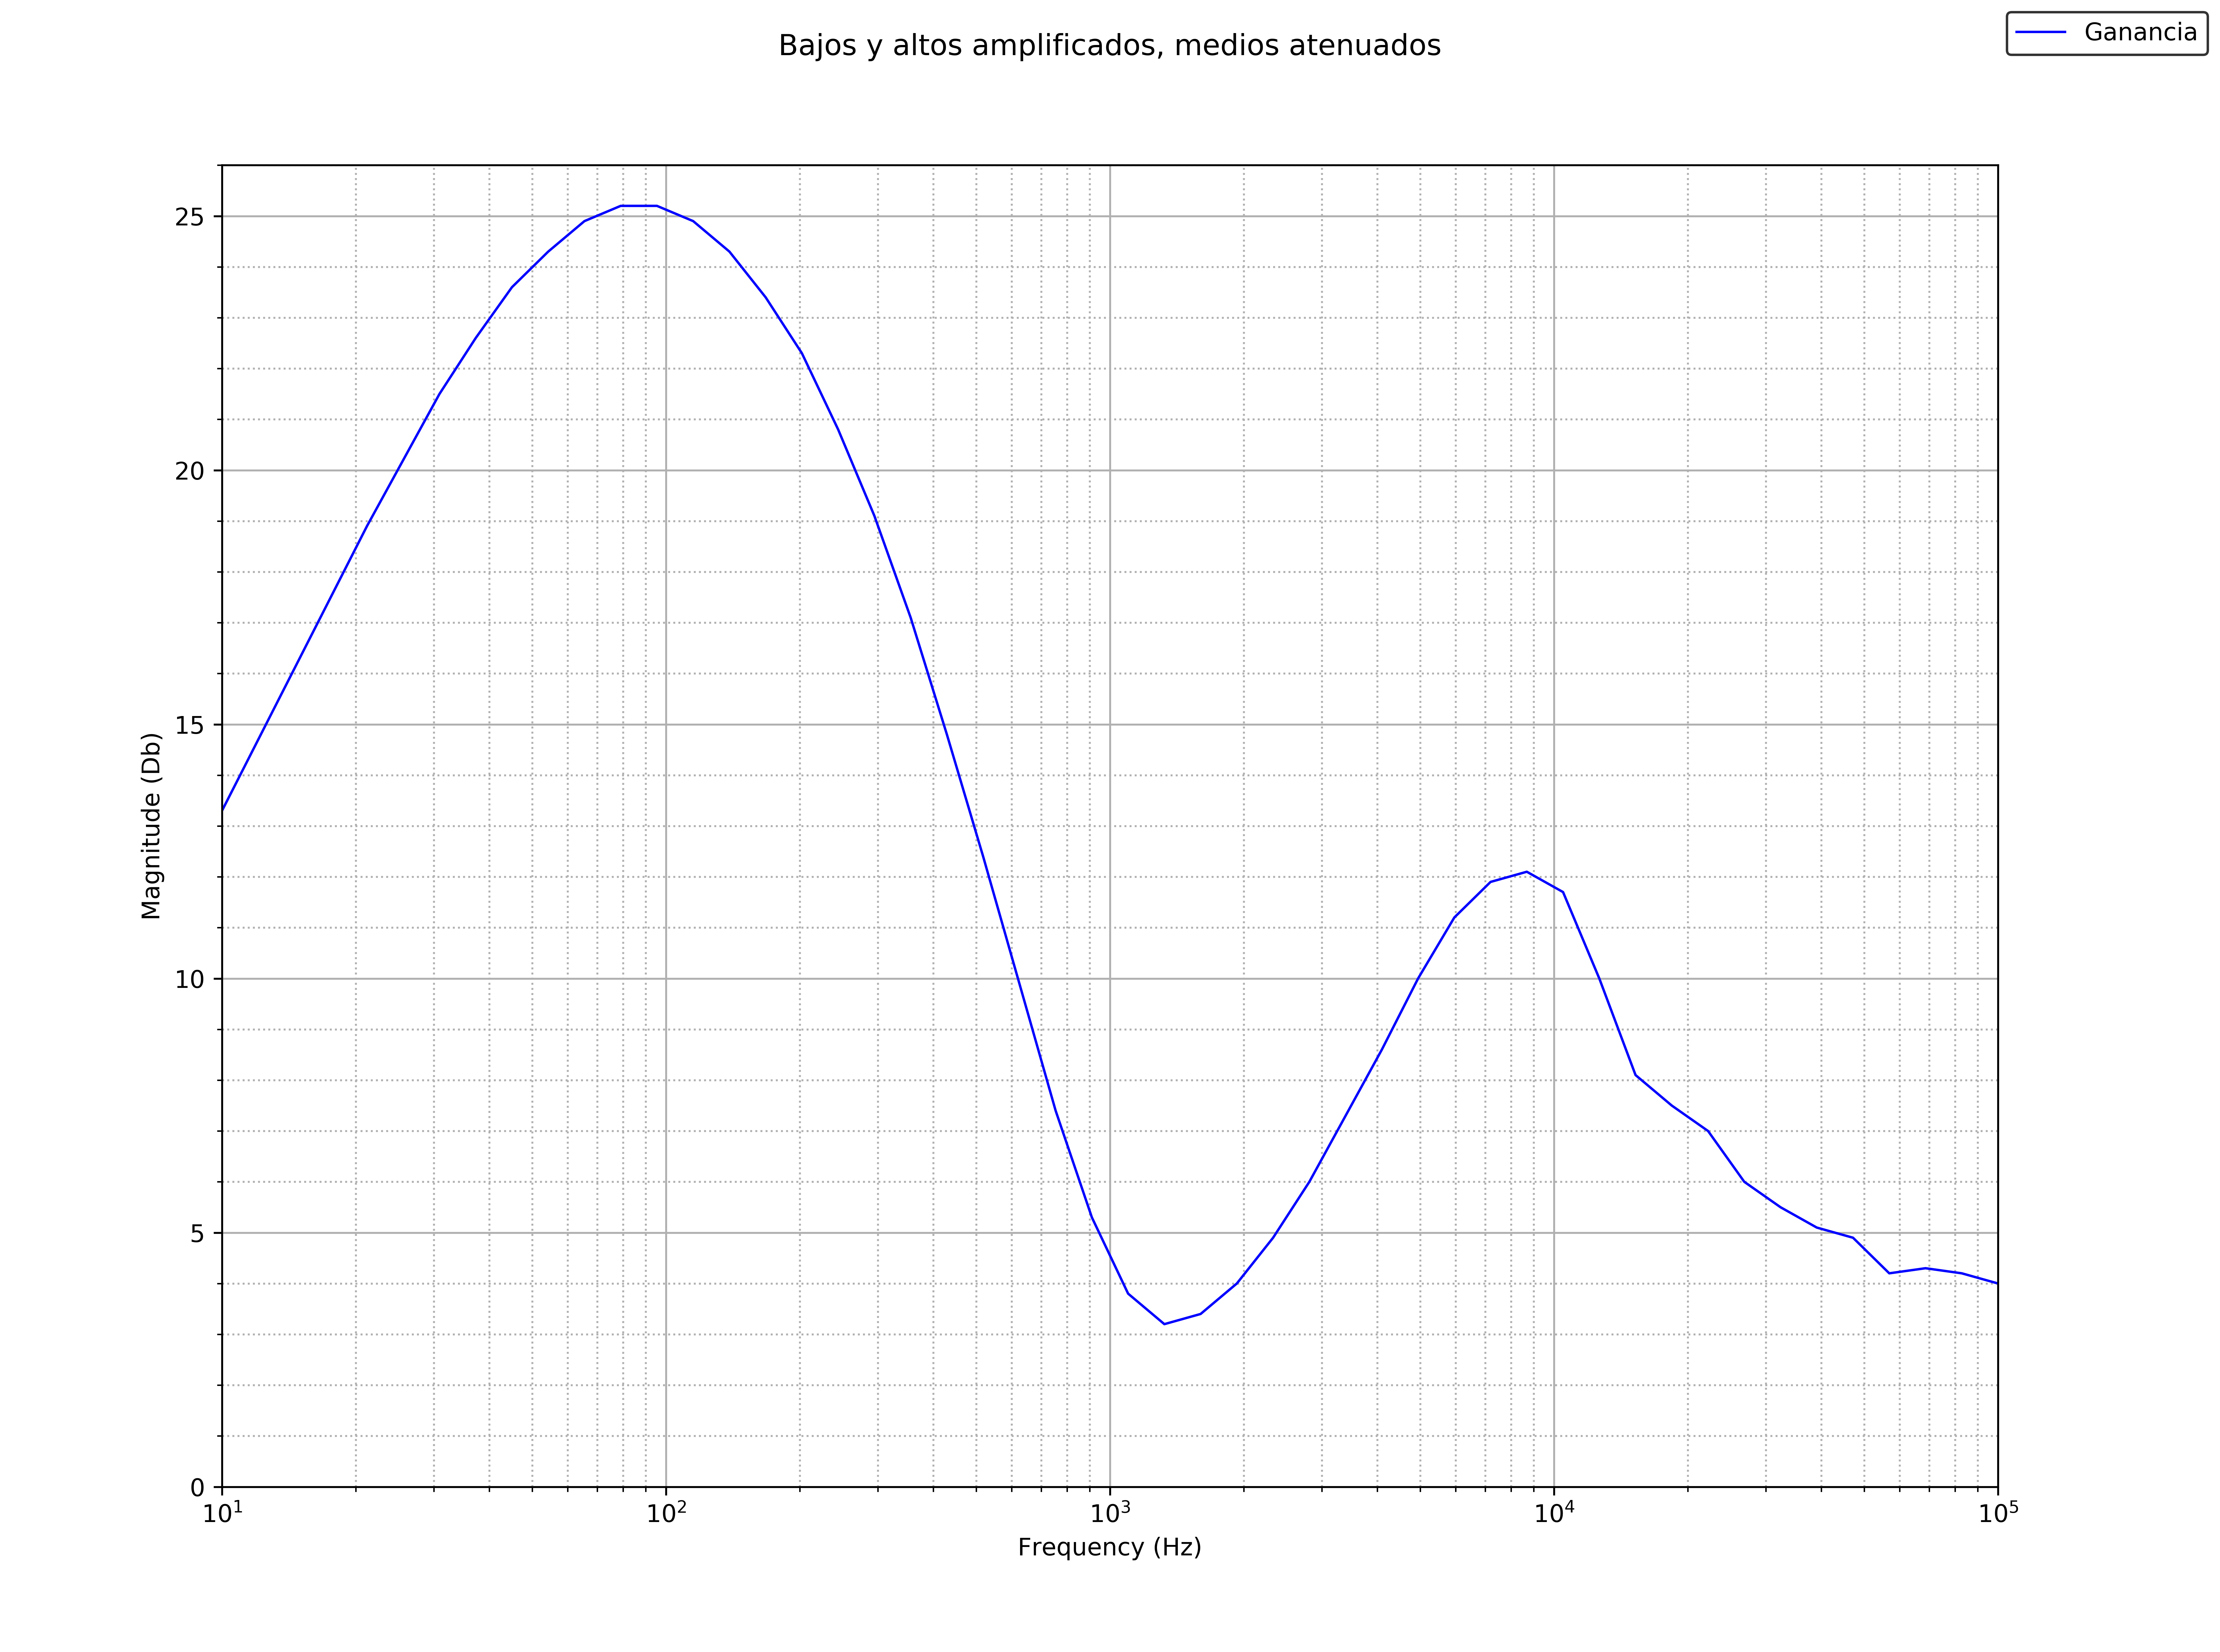
\includegraphics[width=\textwidth]{+B-M+A}
\end{minipage}

\begin{minipage}{0.47\textwidth}
  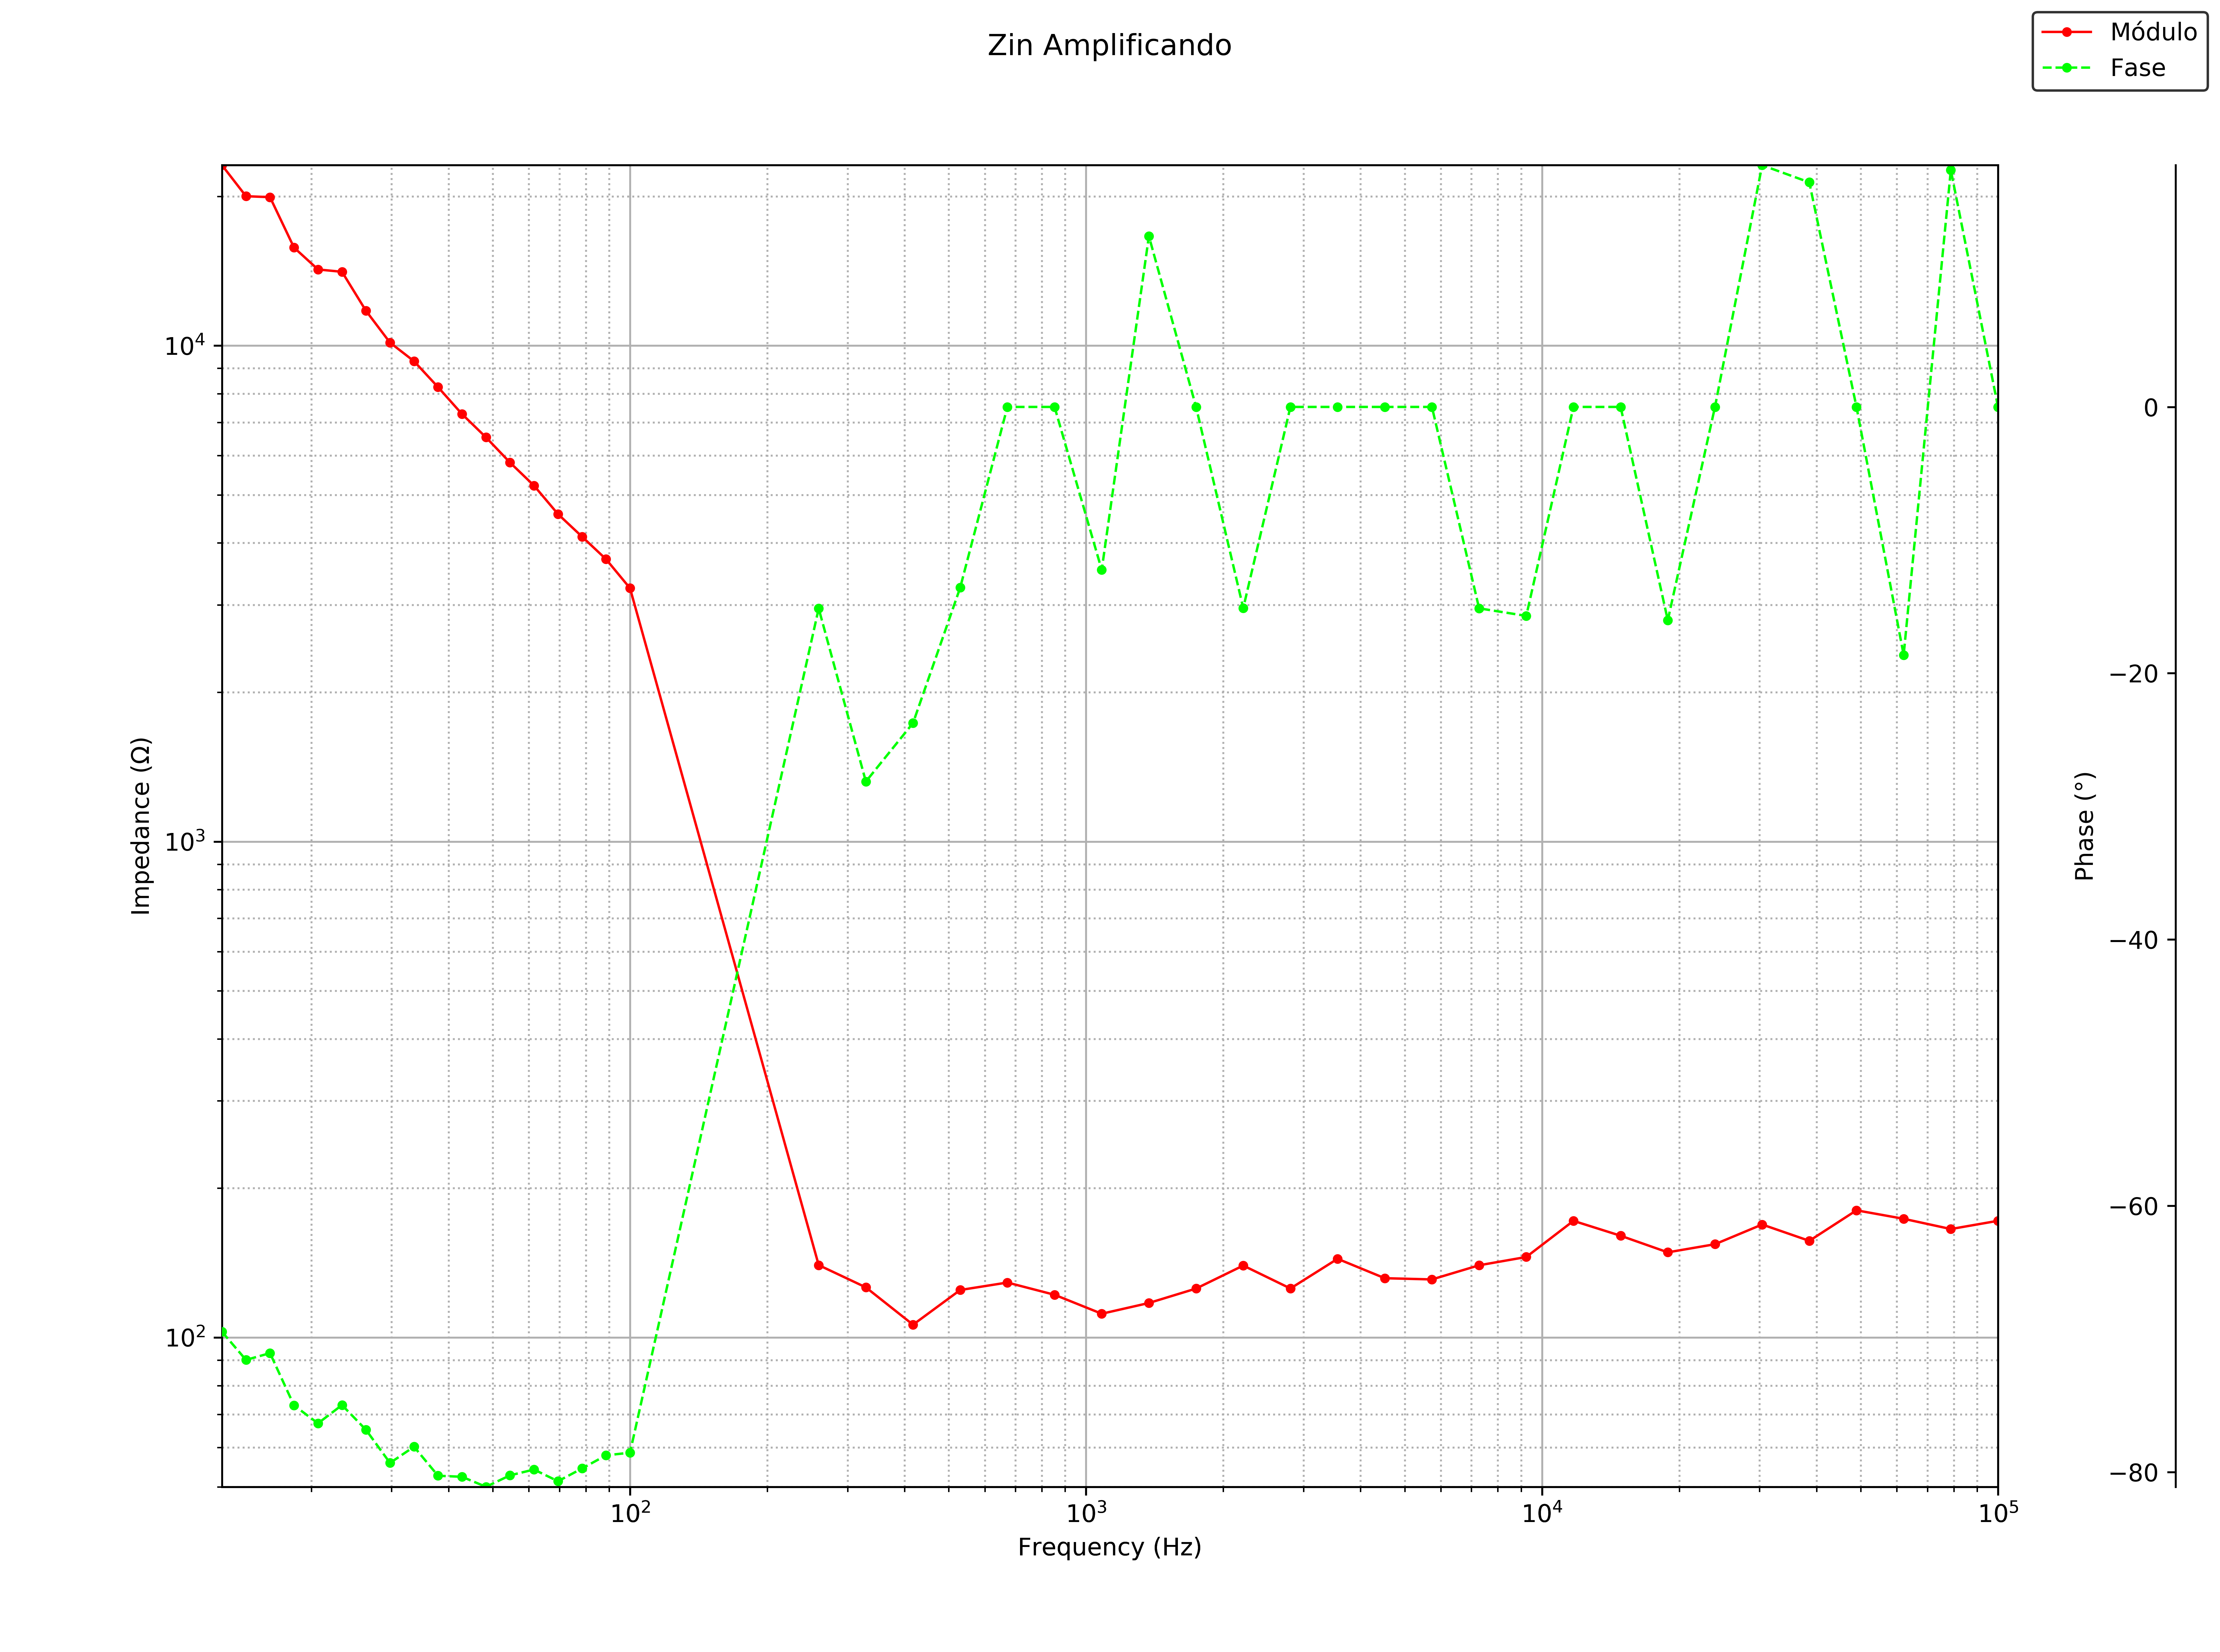
\includegraphics[width=\textwidth]{Zin_H}
\end{minipage}
\hfill
\begin{minipage}{0.47\textwidth}
  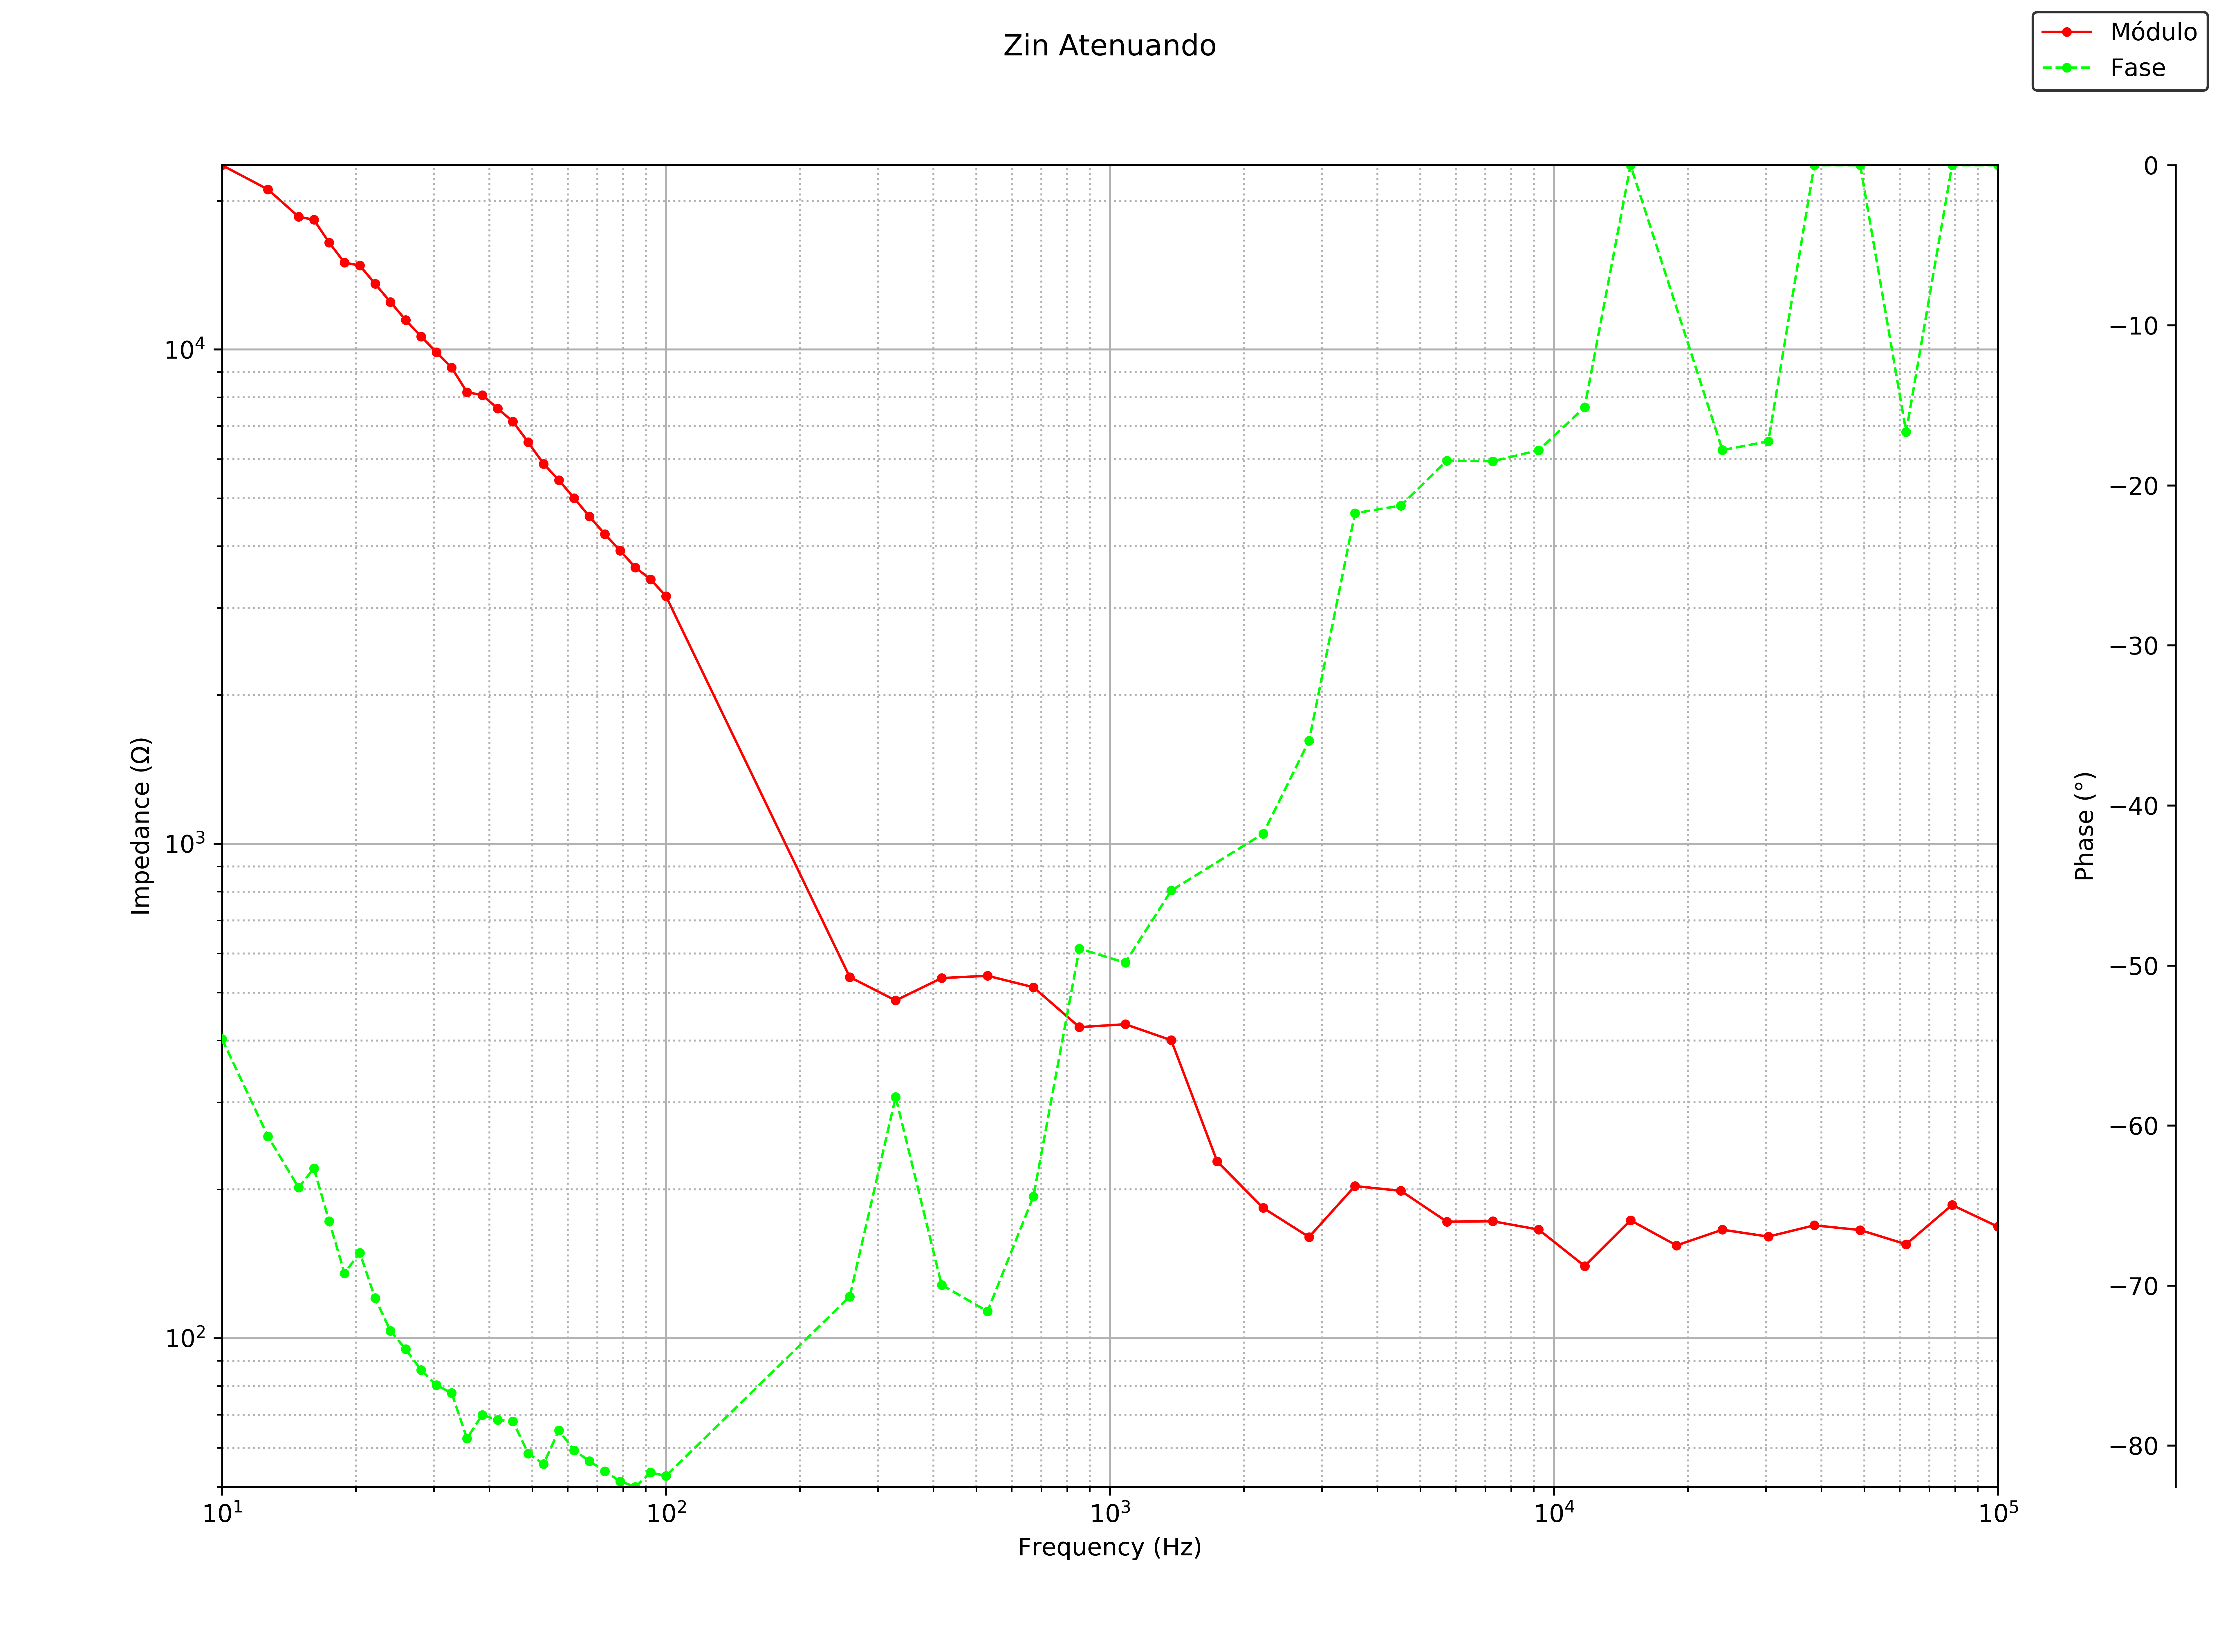
\includegraphics[width=\textwidth]{Zin_L}
\end{minipage}


\newpage
\section{Esquemático}

\begin{figure} [h]
  \centering
  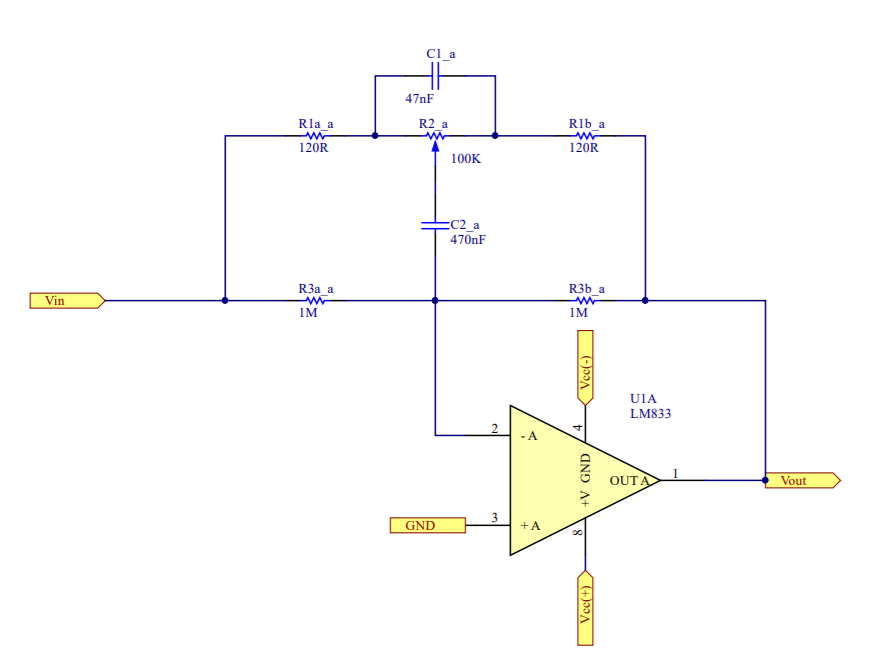
\includegraphics[width=0.8\textwidth, left]{EQL}
  \caption{Circuito ecualizador para una banda (en particular, para las bajas frecuencias)}

\end{figure}

\end{document}



